\begin{figure}[t!]
	\centering
	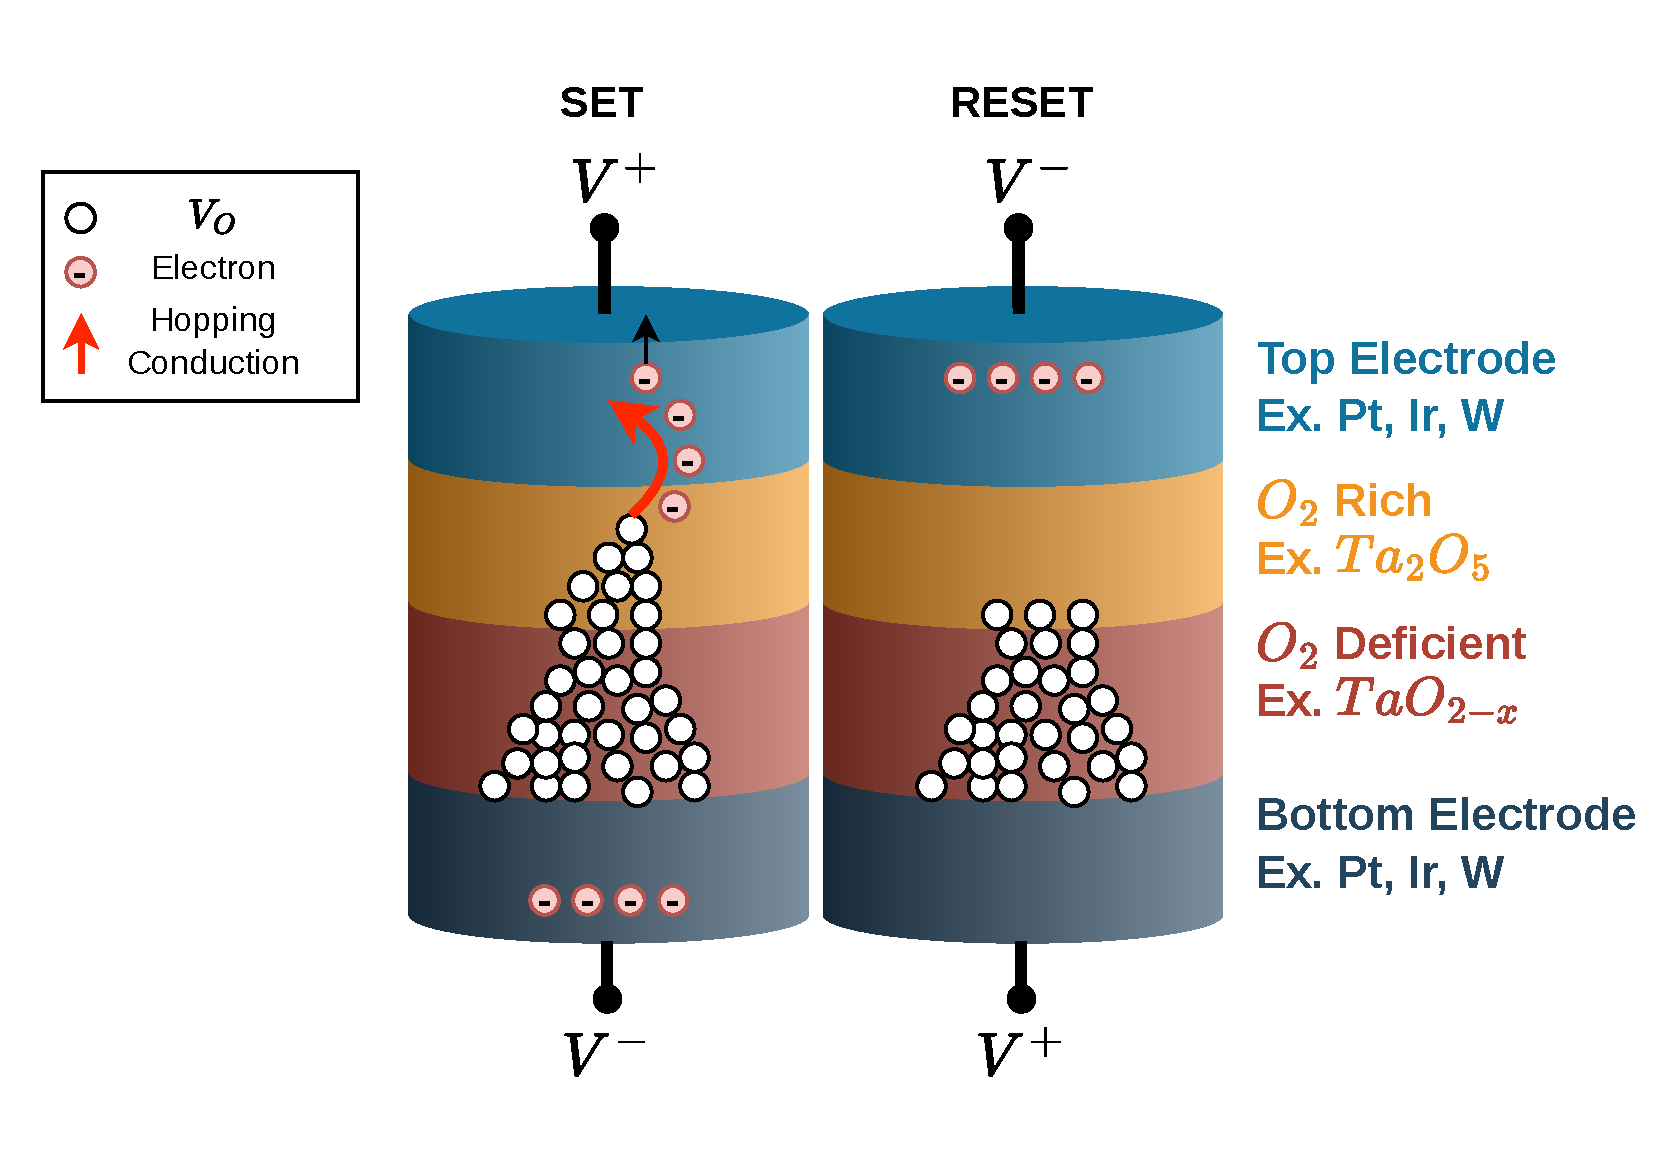
\includegraphics[width=0.9\linewidth]{img/ReRAMDiagram.pdf}
	\caption{Diagram of bipolar OxRAM SET, and RESET physics. The top and bottom electrodes can be either inert (e.g. Pt) or reactive (e.g. W) materials. A switching bi-layer is used to control filament growth. The $O_2$ deficient region acts as a vacancy reservoir. The $O_2$ rich region attracts these vacancies under an electric field. During the set operation, the device is set into its LRS, and hopping conduction under the programming voltage can cause a spike in current, which needs to be limited to avoid damage to the cell.}
	\label{fig:oxram-prog}
\end{figure}